\section{Fermat varieties}\label{sec:fermat}

\subsection{Varieties dominated by CM abelian varieties}

\begin{definition}\label{def:classD}
Let $\cD$ be the class of varieties $X$, possibly disconnected, such that
$H^{*}(X,\QQ)$ is spanned by the images of maps $\Gamma_{*}\colon
H^{*}(B,\QQ)\to H^{*}(X,\QQ)$, where $B$ runs over the abelian varieties of
CM type, the point included, and $\Gamma$ over the algebraic cycles on
$B\times X$.
\end{definition}

\begin{proposition}\label{prop:classD}
\begin{enumerate}[label=\textup{(\roman*)}]
\item Every $X\in\cD$ satisfies \st{F3$'$}. If \st{CM} holds, every
$X\in\cD$ satisfies \HC.
\item $\cD$ contains every abelian variety of CM type and every finite set of
points, and every curve whose Jacobian is of CM type.
\item $\cD$ is closed under finite disjoint unions, under taking connected
components, and under products.
\item If $Z\in\cD$ and $f\colon Z\to X$ is a surjective morphism, then
$X\in\cD$.
\item If $X\in\cD$ and $Y\subseteq X$ is a smooth closed subvariety of
codimension at least two in every component, with $Y\in\cD$, then the
blow-up of $X$ along $Y$ lies in $\cD$.
\end{enumerate}
\end{proposition}

\begin{proof}
(i) By \Cref{lem:dominated}, applied in each degree to finitely many
$\Gamma_{*}$ whose images span, every Hodge class on $X$ is a sum of classes
$\Gamma_{*}\gamma$ with $\gamma$ a Hodge class on an abelian variety of CM
type. Such a class lies in $\Ab^{p}(X)$, and under \st{CM} it is algebraic.

(ii) For $B$ of CM type take $\Gamma$ the diagonal. For a finite set of
points take $B$ a point and $\Gamma$ the points of $X$ one at a time. For a
curve $C$ with Jacobian $J$ of CM type: $H^{0}(C)$ and $H^{2}(C)$ are spanned
by the fundamental class and the class of a point, which are images from the
point, and $H^{1}(C)=\alpha^{*}H^{1}(J)$ for an Abel--Jacobi map
$\alpha\colon C\to J$, and $\alpha^{*}$ is the correspondence given by the
transpose of the graph of $\alpha$.

(iii) A disjoint union: the cohomology is the direct sum, and a cycle on
$B\times X_{i}$ is a cycle on $B\times\bigsqcup_{i}X_{i}$. A connected
component $X'$ of $X$: restriction $H^{*}(X)\to H^{*}(X')$ is surjective and
is the correspondence given by the transpose of the graph of the inclusion,
so composing gives correspondences from the $B$'s onto $H^{*}(X')$. A
product: by the K\"unneth formula $H^{*}(X\times X')$ is spanned by the
classes $\pr^{*}x\cup\pr'^{*}x'$, and if $x=\Gamma_{*}y$ and
$x'=\Gamma'_{*}y'$ then $\pr^{*}x\cup\pr'^{*}x'=\pm(\Gamma\times\Gamma')_{*}
(\pr_{B}^{*}y\cup\pr_{B'}^{*}y')$, where $\Gamma\times\Gamma'$ is a cycle on
$(B\times B')\times(X\times X')$ and $B\times B'$ is of CM type.

(iv) By (iii) we may assume $X$ connected and replace $Z$ by a component
that maps onto $X$. By \Cref{prop:descent} there is a correspondence $\Gamma$
from $Z$ to $X$ with $\Gamma_{*}$ surjective; composing it with the
correspondences that dominate $H^{*}(Z)$ gives correspondences that dominate
$H^{*}(X)$.

(v) By \Cref{prop:blowup} the cohomology of the blow-up is spanned by the
images of correspondences from $X$ and from $Y$; compose them with the
correspondences that dominate $H^{*}(X)$ and $H^{*}(Y)$.
\end{proof}

\subsection{Fermat curves}

\begin{lemma}\label{lem:fermatcurve}
For every $m\ge1$ the Jacobian of the Fermat curve $X^{1}_{m}$ is of CM type.
\end{lemma}

\begin{proof}
For $m\le2$ the curve is rational and the Jacobian is a point. Let $m\ge3$,
let $g=(m-1)(m-2)/2$ be the genus, and use the affine model $u^{m}+v^{m}=1$,
which is isomorphic to $X^{1}_{m}$ over $\CC$. The group $G=\mu_{m}\times
\mu_{m}$ acts by $(\zeta,\zeta')\cdot(u,v)=(\zeta u,\zeta'v)$, and this action
extends to the smooth projective curve. The forms
\[
  \omega_{r,s}=u^{r-1}v^{s-m}\,du,\qquad r,s\ge1,\quad r+s\le m-1,
\]
are holomorphic\footnote{On the affine curve $v^{s-m}du=-v^{s-1}u^{1-m}dv$
shows that $\omega_{r,s}$ has no poles where $u$ or $v$ is finite. At the
$m$ points at infinity, $u$ and $v$ have simple poles and $du$ has a double
pole, so $\omega_{r,s}$ has order $-(r-1)-(s-m)-2=m-1-r-s\ge0$ there.}, and
there are $(m-1)(m-2)/2=g$ of them, so they form a basis of $H^{1,0}$. The
form $\omega_{r,s}$ is an eigenvector of $G$ with character
$(\zeta,\zeta')\mapsto\zeta^{r}\zeta'^{s}$, and distinct pairs $(r,s)$ give
distinct characters, since $1\le r,s\le m-2$. The complex conjugates span
$H^{0,1}$ and have the characters $(-r,-s)=(m-r,m-s)$; since
$(m-r)+(m-s)\ge m+1$, none of these occurs in $H^{1,0}$. So $H^{1}(X^{1}_{m},
\CC)$ is the direct sum of $2g$ lines on which $G$ acts by $2g$ distinct
characters.

Let $E\subseteq\End(H^{1}(X^{1}_{m},\QQ))$ be the image of the group algebra
$\QQ[G]$. It is commutative and semisimple, as a quotient of a commutative
semisimple algebra, and $E\otimes\CC$ is the image of $\CC[G]$, which acts on
each of the $2g$ lines through its own character; since the characters are
distinct, $E\otimes\CC\cong\CC^{2g}$ and $\dim_{\QQ}E=2g$. The elements of $G$
act on the Jacobian, and $H^{1}$ of the Jacobian is $H^{1}$ of the curve, so
$E\subseteq\End(J)\otimes\QQ$. Thus $J$ is of CM type.
\end{proof}

The characters can be grouped into orbits of $(\ZZ/m)^{\times}$, and each
orbit spans the cohomology of an isogeny factor of $J$ with complex
multiplication by a quotient of $\QQ(\mu_{m})$ \cite{KR78}; this is the
classical computation of Weil \cite{Wei52}.

\subsection{The inductive structure}
Fix $m\ge1$ and write $X^{n}=X^{n}_{m}$, the Fermat variety
$x_{0}^{m}+\dots+x_{n+1}^{m}=0$ in $\PP^{n+1}$, for $n\ge0$; thus $X^{0}$ is a
set of $m$ points. Fix $\varepsilon$ with $\varepsilon^{m}=-1$.

\begin{proposition}[Shioda--Katsura \cite{SK79}]\label{prop:sk}
Let $r,s\ge1$, let $Y\subseteq X^{r}\times X^{s}$ be the subvariety
$x_{r+1}=y_{s+1}=0$, which is isomorphic to $X^{r-1}\times X^{s-1}$ and has
codimension two, and let $Z$ be the blow-up of $X^{r}\times X^{s}$ along $Y$.
The rational map $\varphi\colon X^{r}\times X^{s}\dashrightarrow X^{r+s}$,
\[
  \varphi(x,y)=\bigl[x_{0}y_{s+1}:\dots:x_{r}y_{s+1}:\ \varepsilon x_{r+1}y_{0}:
  \dots:\varepsilon x_{r+1}y_{s}\bigr],
\]
is defined exactly off $Y$, and it extends to a surjective morphism
$Z\to X^{r+s}$.
\end{proposition}

\begin{proof}
The image lies in $X^{r+s}$, because
$y_{s+1}^{m}\sum_{i\le r}x_{i}^{m}+\varepsilon^{m}x_{r+1}^{m}\sum_{j\le s}
y_{j}^{m}=-y_{s+1}^{m}x_{r+1}^{m}+x_{r+1}^{m}y_{s+1}^{m}=0$. All coordinates
vanish exactly on $Y$: if $y_{s+1}\ne0$ they force $x_{0}=\dots=x_{r}=0$ and
then $x_{r+1}^{m}=-\sum_{i\le r}x_{i}^{m}=0$, which is impossible; so
$y_{s+1}=0$, and in the same way $x_{r+1}=0$. On the blow-up, on the chart
where $y_{s+1}=t\,x_{r+1}$, the map is $[t x_{0}:\dots:t x_{r}:\varepsilon
y_{0}:\dots:\varepsilon y_{s}]$; here $y_{0},\dots,y_{s}$ do not all vanish,
because otherwise $y_{s+1}^{m}=0$ as well. The other chart is symmetric. So
$\varphi$ extends to a morphism on $Z$ \cite[Lemma~1.2]{SK79}. It is
dominant, since from a general point of $X^{r+s}$ one recovers
$[x_{0}:\dots:x_{r}]$ and $[y_{0}:\dots:y_{s}]$, and then $x_{r+1}$ and
$y_{s+1}$ up to finitely many choices; its image is closed and $X^{r+s}$ is
irreducible for $r+s\ge2$, so it is surjective.\footnote{Shioda and Katsura
show more: the morphism $Z\to X^{r+s}$ is the composite of the quotient by a
cyclic group of order $m$ and a
birational morphism that contracts two disjoint subvarieties of the quotient
\cite[Theorem~1.7]{SK79}. We use only that it is a surjective morphism.}
\end{proof}

\subsection{Proof of \texorpdfstring{\Cref{thm:C}}{Theorem C}}\label{ssec:proofC}

\begin{theorem}\label{thm:fermatD}
Every Fermat variety $X^{n}_{m}$ lies in $\cD$. So do all products of Fermat
varieties of any degrees and dimensions, and every variety onto which such a
product maps surjectively.
\end{theorem}

\begin{proof}
Fix $m$. We show $X^{n}\in\cD$ by induction on $n$. The set of points
$X^{0}$ lies in $\cD$, and so does the curve $X^{1}$, by
\Cref{prop:classD}(ii) and \Cref{lem:fermatcurve}. Let $n\ge2$ and suppose
$X^{k}\in\cD$ for $k<n$. Apply \Cref{prop:sk} with $r=1$ and $s=n-1$. The
product $X^{1}\times X^{n-1}$ and the centre $Y\cong X^{0}\times X^{n-2}$ lie
in $\cD$ by \Cref{prop:classD}(iii); the blow-up $Z$ lies in $\cD$ by
\Cref{prop:classD}(v); and $X^{n}$, the image of $Z$, lies in $\cD$ by
\Cref{prop:classD}(iv). The remaining assertions are
\Cref{prop:classD}(iii) and~(iv).
\end{proof}

\begin{proof}[Proof of \Cref{thm:C}]
Combine \Cref{thm:fermatD} with \Cref{prop:classD}(i).
\end{proof}

The proof shows more than \Cref{thm:C} states: every Hodge class on a
Fermat variety is the image, under an explicit algebraic correspondence, of a
Hodge class on a power of the Jacobians of Fermat curves of the same degree.
\Cref{thm:C} is therefore exactly as strong as \st{CM} for these powers.

\subsection{The Hodge classes of a Fermat variety}\label{ssec:fermathodge}

The group $G_{n}=\mu_{m}^{n+2}/\mu_{m}$ acts on $X^{n}_{m}$ by multiplying
the coordinates, and its characters are the vectors
$a=(a_{0},\dots,a_{n+1})\in(\ZZ/m)^{n+2}$ with $\sum a_{i}=0$. Let
$\mathfrak{A}^{n}_{m}$ be the set of characters with every $a_{i}\ne0$. For
$a\in\mathfrak{A}^{n}_{m}$ write $\langle a\rangle=\sum_{i}\bar a_{i}/m$,
where $\bar a_{i}\in\{1,\dots,m-1\}$ represents $a_{i}$; it is an integer
between $1$ and $n+1$.

\begin{proposition}\label{prop:fermatchars}
\begin{enumerate}[label=\textup{(\roman*)}]
\item The primitive cohomology $H^{n}_{\mathrm{prim}}(X^{n}_{m},\CC)$ is the
direct sum of lines $V(a)$, one for each $a\in\mathfrak{A}^{n}_{m}$, on which
$G_{n}$ acts by pull-back through the character $a$; and $V(a)\subseteq H^{n-q,q}$ with $q=\langle
a\rangle-1$. Hence
\[
  \dim H^{n}_{\mathrm{prim}}=|\mathfrak{A}^{n}_{m}|
  =\frac{(m-1)^{n+2}+(-1)^{n}(m-1)}{m},\qquad
  h^{n-q,q}_{\mathrm{prim}}=\#\{a:\langle a\rangle=q+1\}.
\]
\item Let $n$ be even. The space of primitive Hodge classes, tensored with
$\CC$, is the sum of the lines $V(a)$ for which $\langle ta\rangle=n/2+1$ for
every $t\in(\ZZ/m)^{\times}$.
\end{enumerate}
\end{proposition}

\begin{proof}
(i) By Griffiths' description of the cohomology of a hypersurface by
residues \cite[\S8]{Gri69}, $H^{n-q,q}_{\mathrm{prim}}(X^{n}_{m})$ is
isomorphic to the graded piece of degree $(q+1)m-(n+2)$ of the Jacobian ring
$\CC[x_{0},\dots,x_{n+1}]/(x_{0}^{m-1},\dots,x_{n+1}^{m-1})$, the class of a
monomial $x^{b}$ corresponding to the residue of $x^{b}\Omega/F^{q+1}$, where
$F=\sum x_{i}^{m}$ and $\Omega=\sum(-1)^{i}x_{i}\,dx_{0}\wedge\cdots\widehat{
dx_{i}}\cdots\wedge dx_{n+1}$. That residue is an eigenvector of $G_{n}$ with
character $a=b+(1,\dots,1)$, because $\Omega$ has character $(1,\dots,1)$
and $F$ is invariant. As $b$ runs over the exponents with $0\le b_{i}\le
m-2$, the vector $a$ runs once over the characters with $1\le\bar a_{i}\le
m-1$; the degree condition is $\sum\bar a_{i}=(q+1)m$, that is,
$\langle a\rangle=q+1$, and it forces $\sum a_{i}=0$ in $\ZZ/m$. The count
of $\mathfrak{A}^{n}_{m}$ follows from the recursion
$N_{k}=(m-1)^{k-1}-N_{k-1}$, $N_{1}=0$, for the number $N_{k}$ of $k$-tuples of
nonzero residues with sum zero.

(ii) The eigenspace decomposition is defined over $\QQ(\mu_{m})$, and the
automorphism $\zeta\mapsto\zeta^{t}$ of $\QQ(\mu_{m})$ carries $V(a)$ to
$V(ta)$. So for each orbit $O$ of $(\ZZ/m)^{\times}$ on
$\mathfrak{A}^{n}_{m}$ the sum $\bigoplus_{a\in O}V(a)$ is defined over $\QQ$,
these rational subspaces decompose $H^{n}_{\mathrm{prim}}(X^{n}_{m},\QQ)$, and
the one for $O$ consists of Hodge classes exactly when every $V(a)$, $a\in O$,
has type $(n/2,n/2)$, that is, when $\langle a\rangle=n/2+1$ on $O$. A
rational class with a component on some $V(a)$ has components on the whole
orbit of $a$, so the Hodge classes are the sum of the rational subspaces of
the orbits of this kind.
\end{proof}

For a Fermat surface the Picard number is
$\rho(X^{2}_{m})=1+\#\{a\in\mathfrak{A}^{2}_{m}:\langle ta\rangle=2\ \text{for
all}\ t\in(\ZZ/m)^{\times}\}$, and $h^{1,1}=(2m^{3}-6m^{2}+7m)/3$.
\Cref{fig:fermat} compares the two for $m\le12$. For $m$ prime to $6$,
$\rho=3(m-1)(m-2)+1$, and the N\'eron--Severi group is spanned by the $3m^{2}$
lines on the surface \cite{AS83}; the quartic, quintic and sextic give
$\rho=20$, $37$ and $86$.

\begin{figure}[t]
\centering
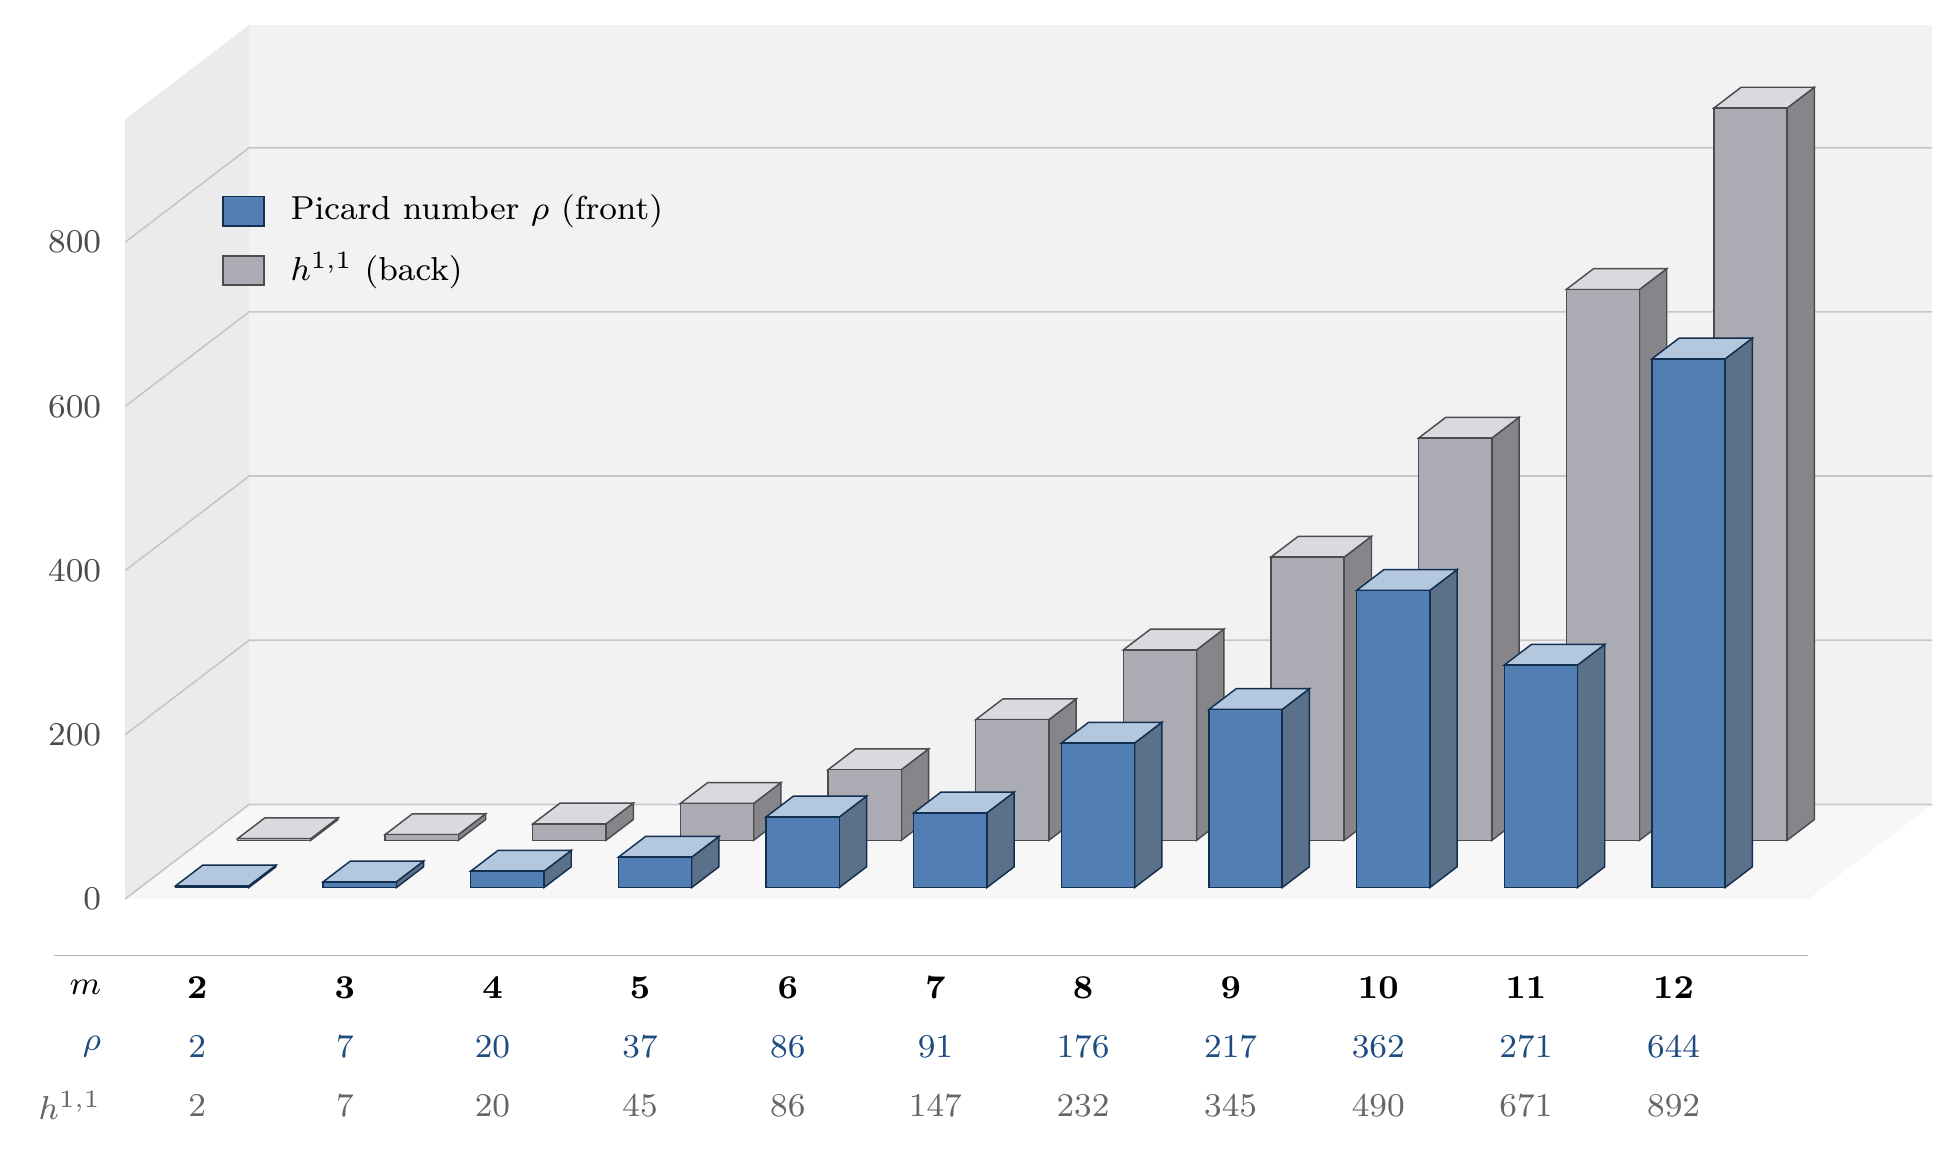
\includegraphics[width=0.92\textwidth]{figures/fig_fermat}
\caption{The Fermat surfaces $X^{2}_{m}$, $2\le m\le12$: the Picard number
$\rho$ (front row) against $h^{1,1}$ (back row), both computed from
\Cref{prop:fermatchars}. On a surface every Hodge class is algebraic
(\Cref{thm:lef11}); the figure shows how the share of $H^{1,1}$ that is
defined over $\QQ$ varies with the arithmetic of $m$. The values of $h^{1,1}$ are recomputed from the Jacobian ring in
Macaulay2 (\Cref{app:checks}).}
\label{fig:fermat}
\end{figure}

\begin{remark}\label{rem:fermatknown}
The Hodge conjecture for $X^{n}_{m}$ is known without hypothesis when $m$ is
prime or $m=4$ \cite{Ran80,Shi79}, when $m\le20$ \cite{Shi79}, and when $m$
is a power of a prime \cite[Corollary~2-3]{Aok87}; see \cite[\S2]{daS21}.
When every prime factor of $m$ exceeds $n+2$, every Hodge character is a
union of pairs \cite[Theorem~A]{Aok83}, and the classes are spanned by linear
subspaces \cite{Ran80,Shi79}; for fourfolds this covers the degrees whose
prime factors are all at least $7$. For fourfolds of degree $m\le100$ prime to
$6$ the conjecture is proved in \cite[Proposition~3.1]{daS21} by a computer
search, and the preprint \cite{Jum26} gives a computer-assisted proof for
fourfolds of odd degree at most $199$. Kang states it for every Fermat
fourfold \cite[Corollary~3.2]{Kan16}, and the preprint \cite{MMRV26}, which
treats all dimensions in degree less than $65$ except $44$, $51$ and $52$,
uses that statement; its proof has the gap described in \Cref{rem:kang}. So
\Cref{thm:F} is new for the degrees $m>199$ prime to $6$ that are divisible by
$5$ and are not powers of $5$, the first of which are $205$, $215$ and $235$,
and its proof, unlike those of \cite{daS21,Jum26}, does not use a computer.
In all these proofs the Hodge classes are written as combinations of the
classes of linear subspaces and of cycles built from them, characters $a$
that split into pairs $a_{i}+a_{j}=0$ corresponding to linear subspaces.
\Cref{thm:C} needs no such decomposition: it moves the whole question to the
Jacobians of Fermat curves. The preprint \cite{OAI26b} announces the Hodge
conjecture on every self-power of a very general member of the family of
diagonal hypersurfaces; the Fermat varieties are special members of that
family.
\end{remark}
